\documentclass[12pt,a4paper]{article}
\usepackage{inverba}
\newcommand{\userName}{Cullyn Newman} 
\newcommand{\class}{BI 216} 
\newcommand{\institution}{Portland State University} 
\newcommand{\thetitle}{\hypertarget{home}{Lab 9 Addendum: Experimental Design}}
\rfoot{\hyperlink{home}{\thepage}}
\usepackage{hyperref}
\hypersetup{
        colorlinks=true,
        linktoc=all,     
        linkcolor=liblue,
        urlcolor=iblue,
    }
    \color{lightmodetext}
    \pagecolor{lightmode}
    \definecolor{under}{HTML}{9e9e9e} 
\begin{document}
Teamates: Molly Parker, Austin Lain, Michael Fernando

\subsection*{Experiment Summary}
\begin{enumerate}[font=\bfseries, wide]
    {\color{under}\item  \textbf{What is the title of your experiment?}  Must be clear and concise while explaining the results of the “sell your project-why it is important” \textbf{(1 pt)}}
    
    Elevation Preferences of Red Pandas in Captivity as Prediction for Survivability in the Wild.

    {\color{under}\item \textbf{ Experiment background:} Provide some background information on the study organism and the experimental conditions that you are testing. \textbf{(2 pts)}}
    
    \textit{Following backround is in large part from Panth, 2011: Feeding Ecology, Habitat Preference and Distribution of Red Panda (Ailurus fulgens fulgens) in Dhopatan Hunting Reserve, Nepal}

    \begin{quotation}
        Red panda are found throughout the Himalayan Mountains between 2,200 and 4,800m in elevation, in northern Burma and the districts of western Sichuan and Yunnan. (Roberts and Gittleman, 1984).

        Red panda's activity changes throughout the year based on the temperature, feeding regimes, and the presence of young. They migrate vertically with changes in season. They move upwards for getting direct sunlight in winter and move downward to dense forest of the streamside to escape from direct sunlight during the summer (Panthi, 2009). They are solitary normally. Red pandas are most active at dusk, dawn, and during the night. Movement on the ground is done by a slow, cross-extension gait, and faster bounding or trotting. Red pandas generally sleep in nests made in evergreens.
    
        Habitat loss and fragmentation threaten the red panda throughout its range (Yonzon et al. 1991). To get a better understanding why, we deiced to observe red pandas to see what preference they might have to see how loss of habitat might affect their essential functions.
    \end{quotation}
  \newpage 
    {\color{under}\item What is your research question? \textbf{(0.5 pt)}}

    Do red pandas prefer to spend more time on elevated surfaces or ground surfaces? What activities do they spend in each place? How might deforestation impact them?

    {\color{under}\item What is your hypothesis? \textbf{(0.5 pt)}}
    
    Red pandas will spend more time on elevated surfaces than on ground surfaces and a majority of essential life activities will take place on elevated surfaces.

\end{enumerate}

\subsection*{Materials and Methods}

\begin{enumerate}[font=\bfseries, wide, resume]
    {\color{under}\item What materials did you use? \textbf{(1 pt)}}
    
    Two zoo's webcams were used to observe the red pandas: \href{https://www.youtube.com/watch?v=m3z2AZ5atjU}{Oklahoma City Zoo} and \href{https://www.youtube.com/watch?v=_5_oHPJDDOM}{Trevor Zoo in New York}.

    {\color{under}\item How many organisms did you use? \textbf{(1 pt)}}
    
    The Oklahoma City Zoo is home to two adult red pandas and their two offspring (9 months old each) and the Trevor zoo is home to two adult pandas. Each observation window will be the activity of one panda.
    
    {\color{under}\item  Copy and paste your ethogram below. Provide a figure caption. \textbf{(0.5 pt)}}

    \begin{figure}[h]
        \centering
        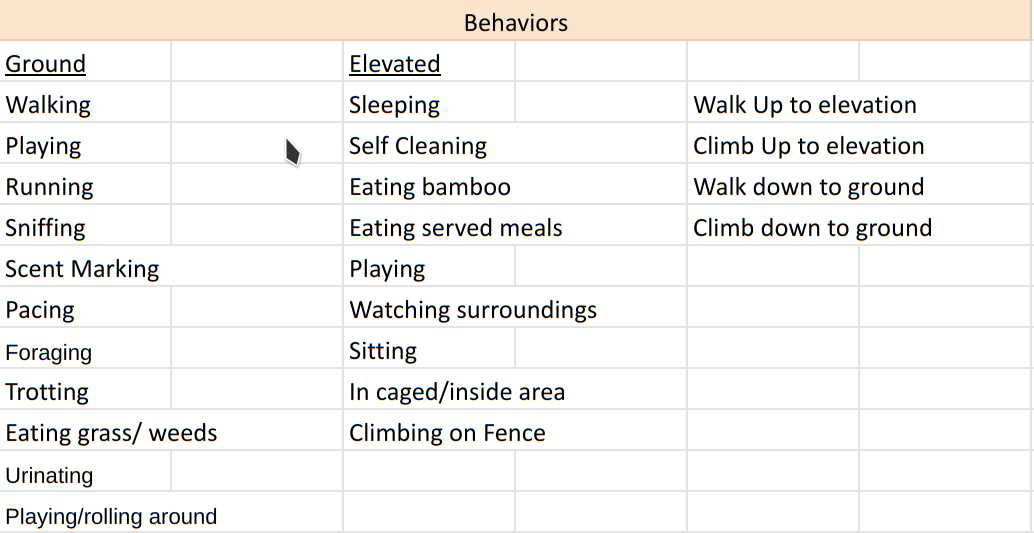
\includegraphics[width=\linewidth]{images/ectogram.png}
        \caption{Ethogram of red panda's behaviors generated from observations from red pandas in captivity Trevor Zoo and OKC Zoo.}
    \end{figure}
\newpage 

    {\color{under}\item How did you execute your experiment?  \textbf{(0.5 pt)}}

    Scan sampling was used to measure time the red pandas spent in various locations. If less than a minute was observed it was not recorded. Camera was not under our control and some safe assumptions were made between breaks in Trevor Zoo as camera panned out of view momentarily (less than one min). 

    In oklahoma city the camera was static, but same methods were used if pandas momentarily (less than one min) left the view. 

    Time varied, and lived redording could be skippet ahead until pandas were in view. Overall, about 1 hour of time on screen was recorded if observations were made that day.
    
    {\color{under}\item  How did you analyze your data? What statistical test did you use? \textbf{(0.5 pt)}}

    We used a statistical T-test to determine if there waws a significant time spent on elevated surfaces versus the ground. Essential life behaviors will be tracked in determined where majority of the time was spent by comparing total time percentages in relevant locations.

   \textbf{Results:} Inconclusive.

   \textbf{OKC zoo:} P-Value = 0.0119, T-value = 2.9590---Significant and suggests hypothesis is invalid.

    \textbf{Trevor zoo:} P-Value = 0.0788, T-value = 1.8962---Not Significant

    \textbf{Totals:} P-Value = 0.9242, T-value = 0.0960---Not Significant: Failure to reject null hypothesis.
\end{enumerate}
\newpage
\subsection*{Results}
\begin{enumerate}[font=\bfseries, wide, resume]
    {\color{under}\item Report your data. Add at least one data table and graph. \textbf{(1.5 pt)}}
    \begin{figure}[h]
        \centering
        \caption{Table showing recorded data of observations between the locations}
        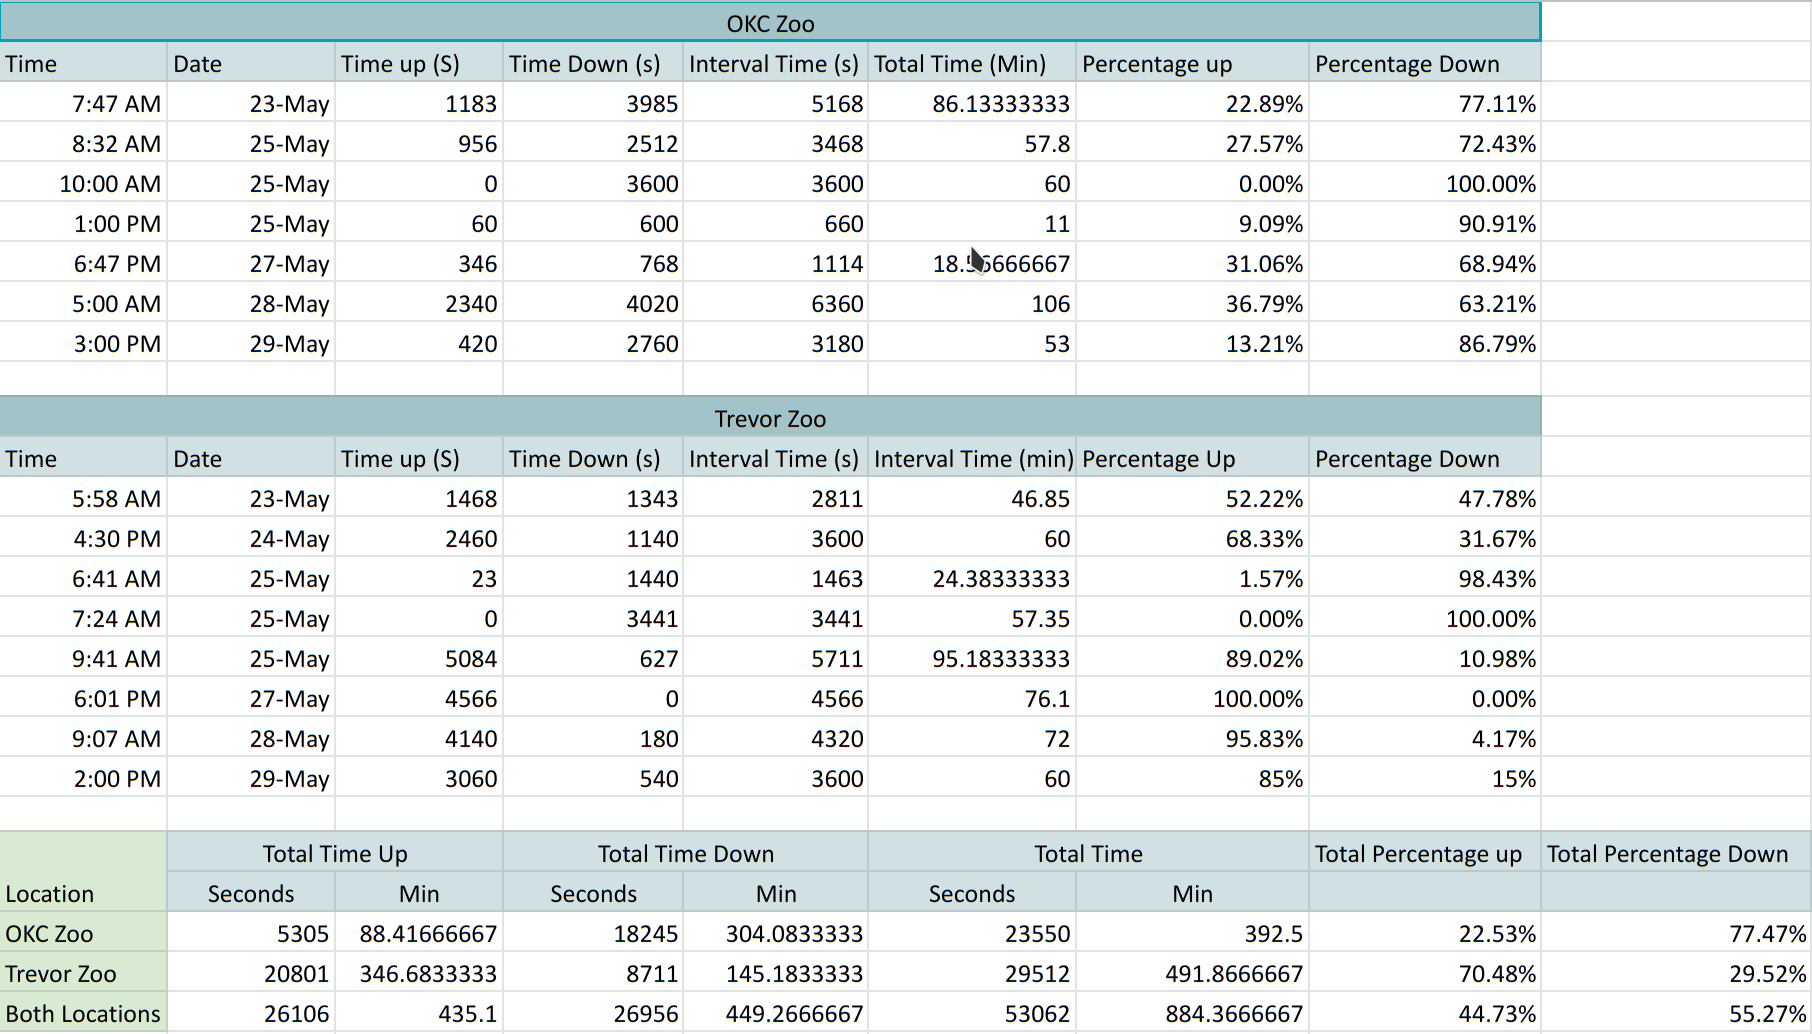
\includegraphics[scale=0.29]{images/tab-9.png}
    \end{figure}
    \begin{figure}[h]
        \centering
        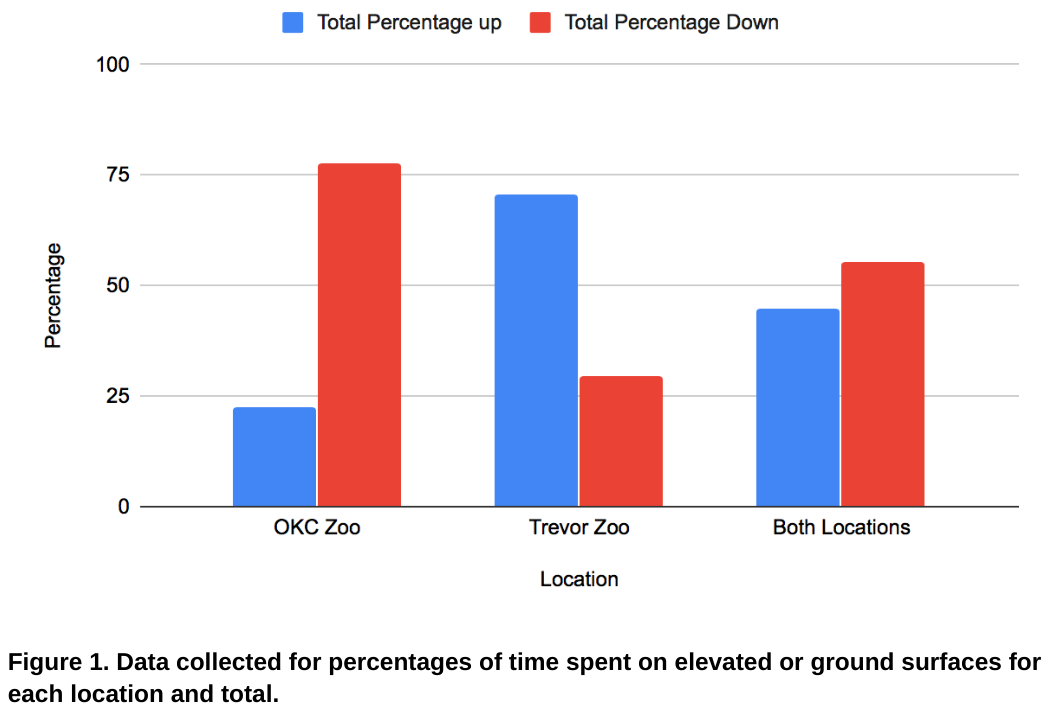
\includegraphics[scale=0.38]{images/fig-9-1.png}
        \caption{Percentage of time spent in relevant location during observations, as well as total.}
    \end{figure}
    \begin{figure}[ht]
        \centering
        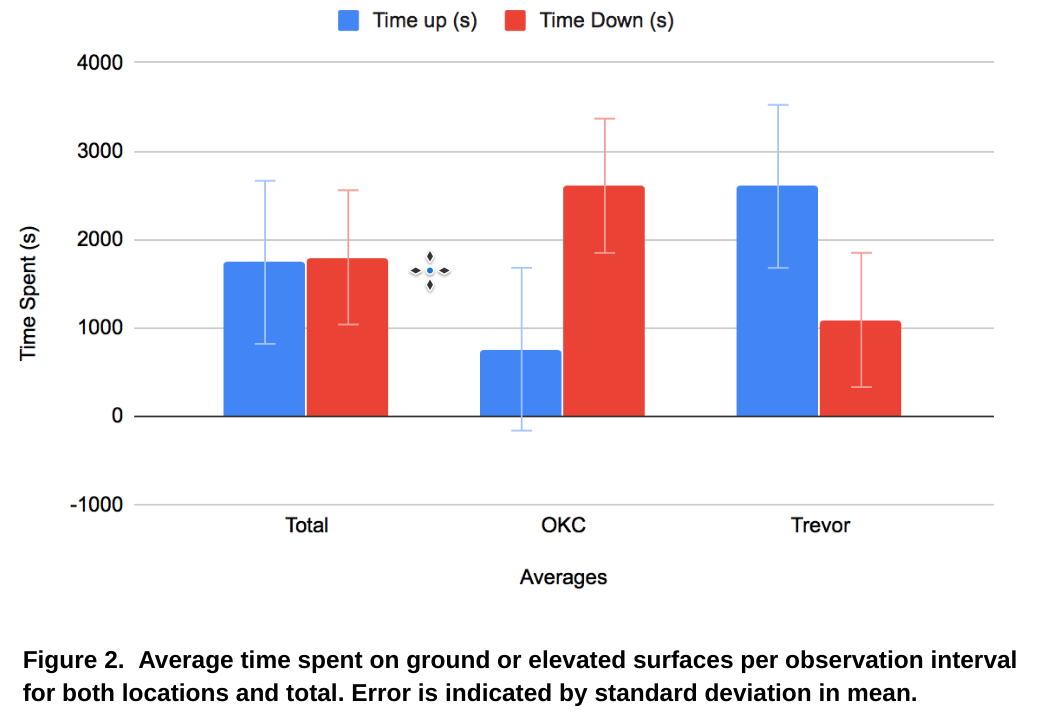
\includegraphics[scale=0.38]{images/fig-9-2.png}
        \caption{Average time spent on ground or elvated surfaces. Error indiated by standard deviation in mean.}
    \end{figure}
\end{enumerate}   
\newpage
\subsection*{Data Interpretation}    
\begin{enumerate}[font=\bfseries, wide, resume]

    {\color{under}\item Interpret your data and statistics, note any flaws in the design. \textbf{(1.5 pt)}}

    Inconclusive. No significant results were obtained, data between locations were contradictory. Cameras at zoo made it extremely difficult to track pandas, much of the time they were not even visible. 
    
    No strong evidence for preference was found. Also, lift in captivity may be vastly different from natural habitat behaviors. Futhermore, even the way each observer was recording data was different, and much estimation was done on certain occasions.

    {\color{under}\item Why did you conduct this experiment? What did you learn? \textbf{(0.5 pt)}}

    Red pandas are cute. We Wanted to see if any information on preferences would help advocate for conservation policies as they are endangered.

    {\color{under}\item Suppose you repeat this experiment, how would you alter your methods? Make suggestions for “next steps”. \textbf{(0.5 pt)}}

    Easily go out to observe them in natural habitat. Any observations in captivity are almost certainly inconclusive and heavily biased. Very little can be done with out real effort.
\end{enumerate}

\subsection*{Works Cited}
\begin{enumerate}[font=\bfseries, wide, resume]

{\color{under}\item Lists your sources \textbf{(0.5 pt)}}

Panthi, S. A. R. O. J. (2011). Feeding ecology, habitat preference and distribution of red panda (Ailurus fulgens fulgens) in Dhopatan Hunting Reserve, Nepal.

Panthi, S. 2009. Status of Ailurs fulgens (Red Panda) in Dhorpatan Hunting Reserve. DHR office, Baglung, Nepal.

Yonzon, P., Jones. R., \& Fox, J. 1991. Geographic Information Systems for assessing Habitat \& Estimating population of red pandas in Langtang National Park, Nepal. Ambio. 20 (7) 285-288.

Roberts M.S., Gittleman, J.L. (1984). Ailurus fulgens. Mammalian Species. 222: 1- 8.
\end{enumerate}
\end{document}